\begin{center}
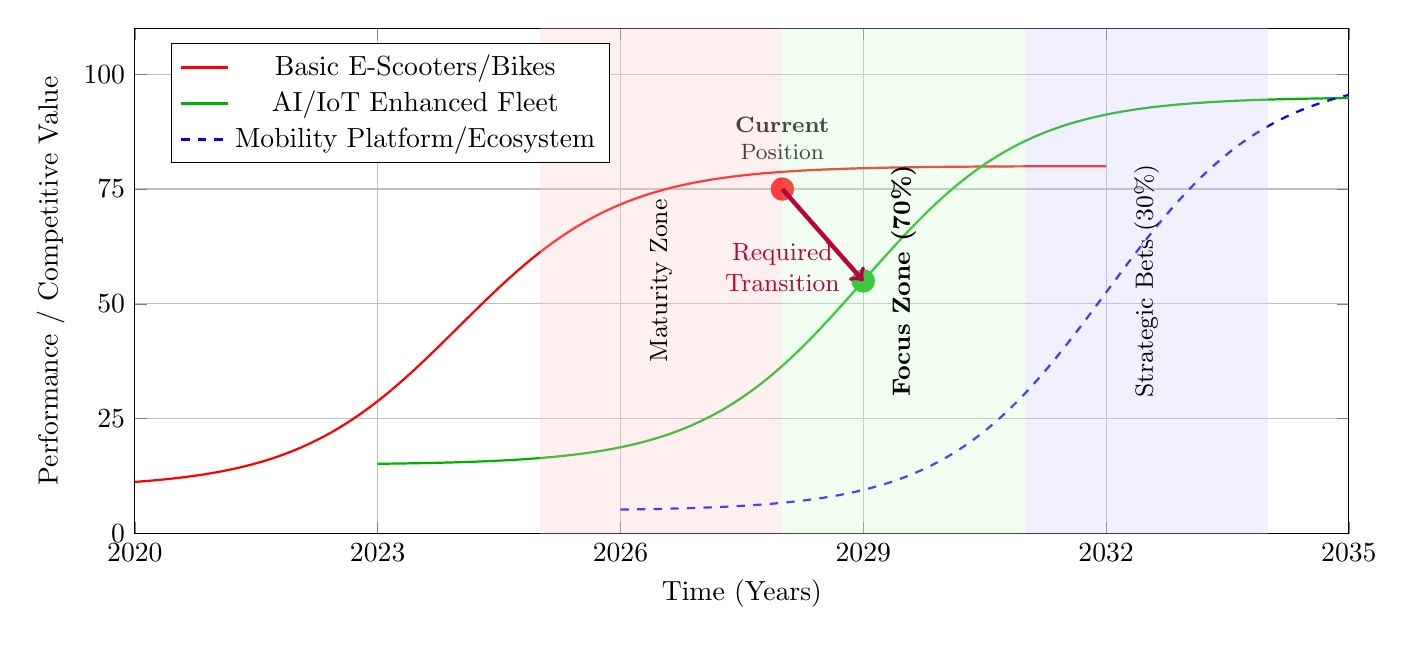
\begin{tikzpicture}
\begin{axis}[
    width=17cm,
    height=8cm,
    xlabel={Time (Years)},
    ylabel={Performance / Competitive Value},
    xmin=0, xmax=15,
    ymin=0, ymax=110,
    xtick={0,3,6,9,12,15},
    xticklabels={2020,2023,2026,2029,2032,2035},
    ytick={0,25,50,75,100},
    grid=major,
    legend pos=north west,
    ylabel style={align=center}
]

% First S-curve: Basic E-mobility (mature)
\addplot[
    domain=0:12,
    samples=100,
    color=red,
    thick
] {70/(1+exp(-1*(x-4))) + 10};
\addlegendentry{Basic E-Scooters/Bikes}

\node[circle, fill=red, inner sep=3pt] at (axis cs:8,75) {};
\node[align=center, font=\footnotesize] at (axis cs:8,86) {\textbf{Current}\\Position};

% Second S-curve: AI/IoT Enhanced (growing)
\addplot[
    domain=3:15,
    samples=100,
    color=green!70!black,
    thick
] {80/(1+exp(-1*(x-9))) + 15};
\addlegendentry{AI/IoT Enhanced Fleet}

\node[circle, fill=green!70!black, inner sep=3pt] at (axis cs:9,55) {};

% Third S-curve: Platform/Ecosystem (emerging)
\addplot[
    domain=6:15,
    samples=100,
    color=blue,
    thick,
    dashed
] {95/(1+exp(-1*(x-12))) + 5};
\addlegendentry{Mobility Platform/Ecosystem}

% Investment zones
\fill[red!20, opacity=0.3] (axis cs:5,0) rectangle (axis cs:8,110);
\node[align=center, font=\small, rotate=90] at (axis cs:6.5,55) {Maturity Zone};

\fill[green!20, opacity=0.3] (axis cs:8,0) rectangle (axis cs:11,110);
\node[align=center, font=\small, rotate=90] at (axis cs:9.5,55) {\textbf{Focus Zone (70\%)}};

\fill[blue!20, opacity=0.3] (axis cs:11,0) rectangle (axis cs:14,110);
\node[align=center, font=\small, rotate=90] at (axis cs:12.5,55) {Strategic Bets (30\%)};

% Transition arrow
\draw[->, ultra thick, purple] (axis cs:8,75) -- (axis cs:9,55);
\node[align=center, font=\small, purple] at (axis cs:8,58) {Required\\Transition};

\end{axis}
\end{tikzpicture}
\end{center}